\begin{figure}[!p]
\centering
\resizebox{\linewidth}{!}{\sffamily
{(a)} \begin{tabular}{c|c|c|c|c|c|c|c}
\texttt{\#70} (184 nt) & Boltzmann prob. & ensemble defect & struct. distance & energy gap & & & \\
``Pokeball'' & $p(\vecystar \mid \vecx)$$(\uparrow)$ & \NED$(\vecx, \vecystar)$$(\downarrow)$ & $d(\MFE(\vecx), \vecystar)$$(\downarrow)$ & \DDG$(\vecx, \vecystar)$$(\downarrow)$ & is \MFE & is uMFE & designable \\
\hline
EliteDesign ($N=500$) & \textbf{0.8428} & \textbf{0.0030} & \textbf{0} & \textbf{0.0 kcal/mol} & \textbf{Yes} & \textbf{Yes} & \multirow{2}{*}{Yes} \\
SamplingDesign & 0.6802 & 0.0115 & \textbf{0} & \textbf{0.0 kcal/mol} & \textbf{Yes} & \textbf{Yes} & \\
\hline
Probability ceiling & 0.8890 & --- & --- & --- & --- & --- & --- \\
\end{tabular}}\\[5pt]
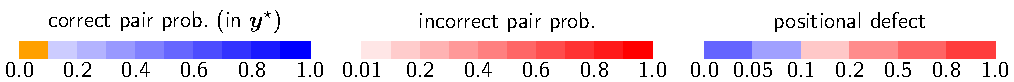
\includegraphics[width=0.9\linewidth]{figures/structures/legend}\\[3pt]
{\sffamily\small
(b) \MFE structure of EliteDesign ($N=500$) ($=$ \vecystar)\\[1pt]
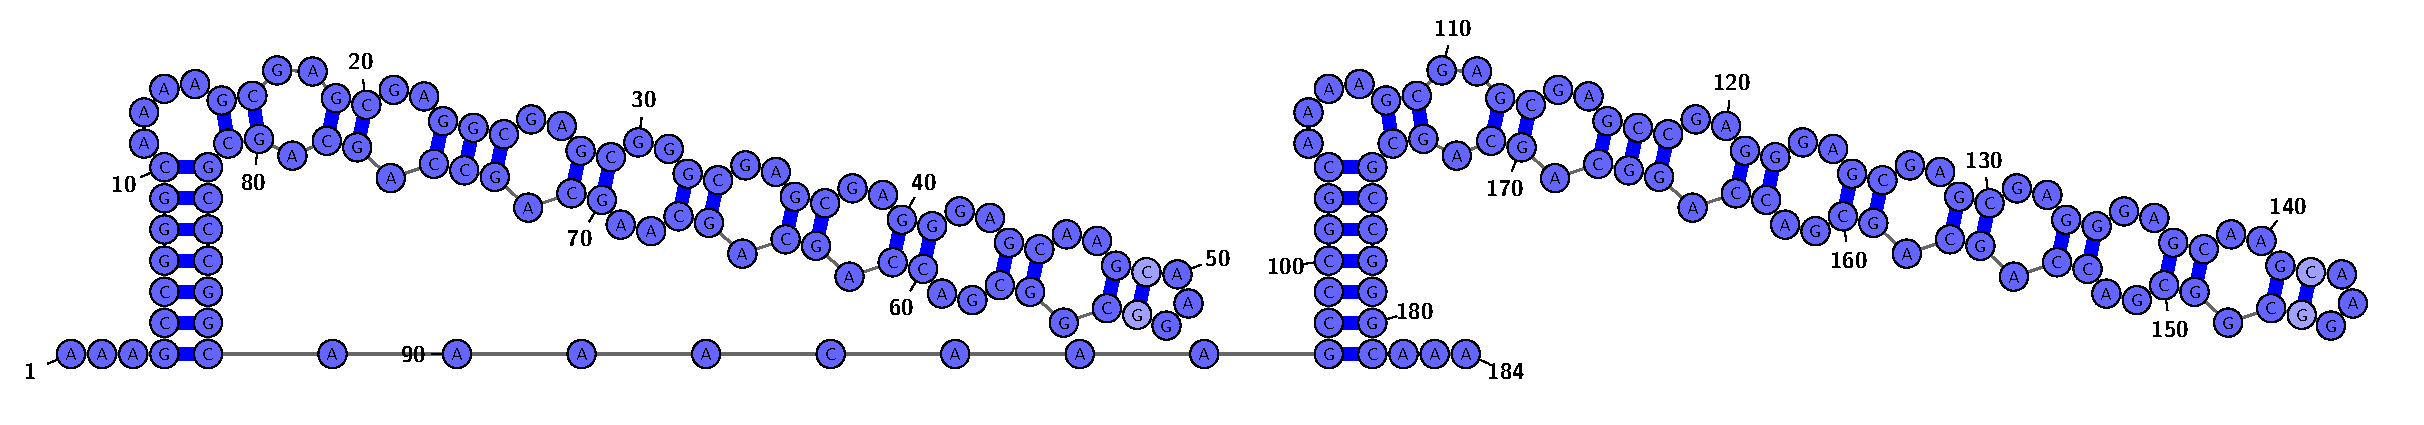
\includegraphics[width=0.98\linewidth]{figures/structures/structure_70_elite}\\[3pt]
(c) \MFE structure of SamplingDesign ($=$ \vecystar)\\[1pt]
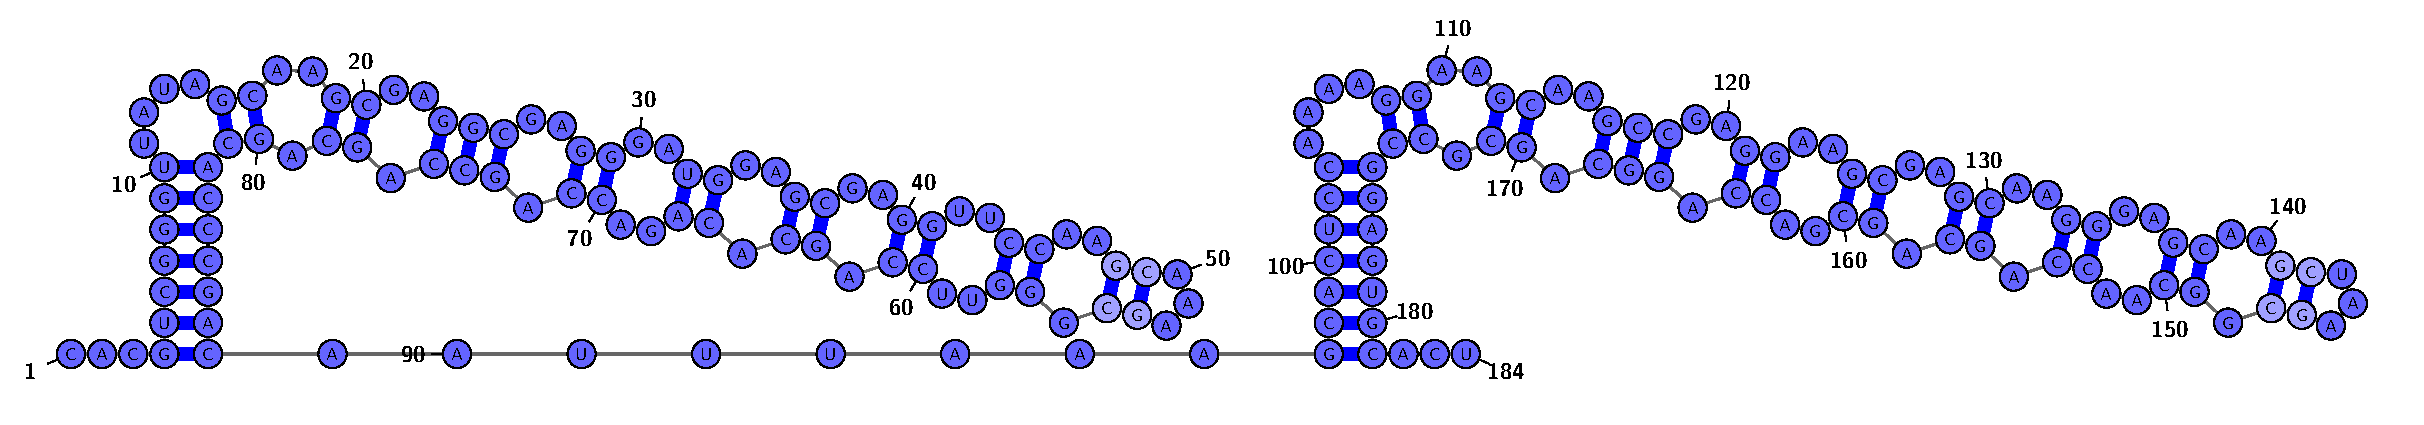
\includegraphics[width=0.98\linewidth]{figures/structures/structure_70_sampling}\\[3pt]
\begin{tabular}{@{}c@{\hspace{0.02\linewidth}}c@{}}
(d) Base-pairing probabilities, EliteDesign ($N=500$) & (e) Base-pairing probabilities, SamplingDesign \\[1pt]
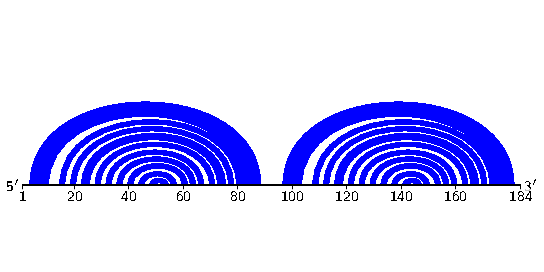
\includegraphics[width=0.49\linewidth]{figures/structures/arcs_70_elite} &
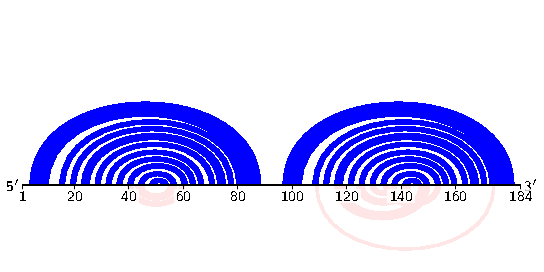
\includegraphics[width=0.49\linewidth]{figures/structures/arcs_70_sampling}
\end{tabular}}
\caption{This figure shows the sequences with the highest Boltzmann probability from EliteDesign ($N=500$) and SamplingDesign on Puzzle \texttt{\#70} (``Pokeball''), which is a designable puzzle. (a) The scores of each design and a probability upper bound on $p(\vecystar\mid\vecx)$~\citep{zhou2026}. (b)--(c) The MFE structure of each design, which is \vecystar. Nucleotides are colored by positional defect. For these MFE predictions, all pairs also belong to \vecystar, and the shade of blue indicates the probability, with darker being higher. (d)--(e) Base-pairing probabilities, where blue arcs are the pairs that match between a structure $\vecy'$ in the ensemble and \vecystar, orange arcs are matching pairs with a probability under 0.1, and red arcs are the pairs of $\vecy'$ that do not match \vecystar. Darker arcs have higher probability.}
\label{fig:eterna-structure-70}
\end{figure}
